\clearpage
%\begin{algorithm}[H]
%    \DontPrintSemicolon
%    \SetKwFunction{FLinkmodel}{Linkmodel}
%    \SetKwProg{Fn}{Function}{}{}
%
%    \Fn{\FLinkmodel{links}}{
%        \ForEach{$l \in $ links}{
%            neighbours $\leftarrow$ findNeighbourhood($l$)\;
%            \ForEach{$neighbour \in neighbours$}{
%                C $\leftarrow r(l, neighbour)$ // The autocorrelation %function\;
%
%                $\Sigma \leftarrow \sigma^2$C // The covariance matrix\;
%            }
%        }
%    }
%
%    \caption{Pseoducode for the linkmodel}
%    \label{algo:linkmodel}
%\end{algorithm}

\paragraph{Link Model}
\medbreak


\begin{tikzpicture}
    \begin{axis}[
            no markers, axis lines*=left,
            enlargelimits=false, clip=false, axis on top,
            xlabel=Average RSSI, ylabel=Probability density,
            height=12cm, width=12cm,
            domain=-40:40,
            % xtick={4,6.5}, ytick=\empty,
            grid=major
        ]

        \addplot[very thick, solid, cyan!50!black, samples=100] {gauss( 0.6787755836206504, 10.929221904852618)};
        \addlegendentry{100 - 150};

        \addplot[very thick, dashed, cyan!50!black, samples=100] {gauss(1.4021184158785516, 8.079011133504437)};
        \addlegendentry{300 - 350};

        \addplot[very thick, loosely dashed, cyan!50!black, samples=100] {gauss(1.9580853586687728, 5.444581964307228)};
        \addlegendentry{500 - 550};

        \addplot[very thick, dotted, cyan!50!black, samples=100] {gauss(-0.32184116101942706, 4.431214224678553)};
        \addlegendentry{650 - 700};
    \end{axis}
\end{tikzpicture}

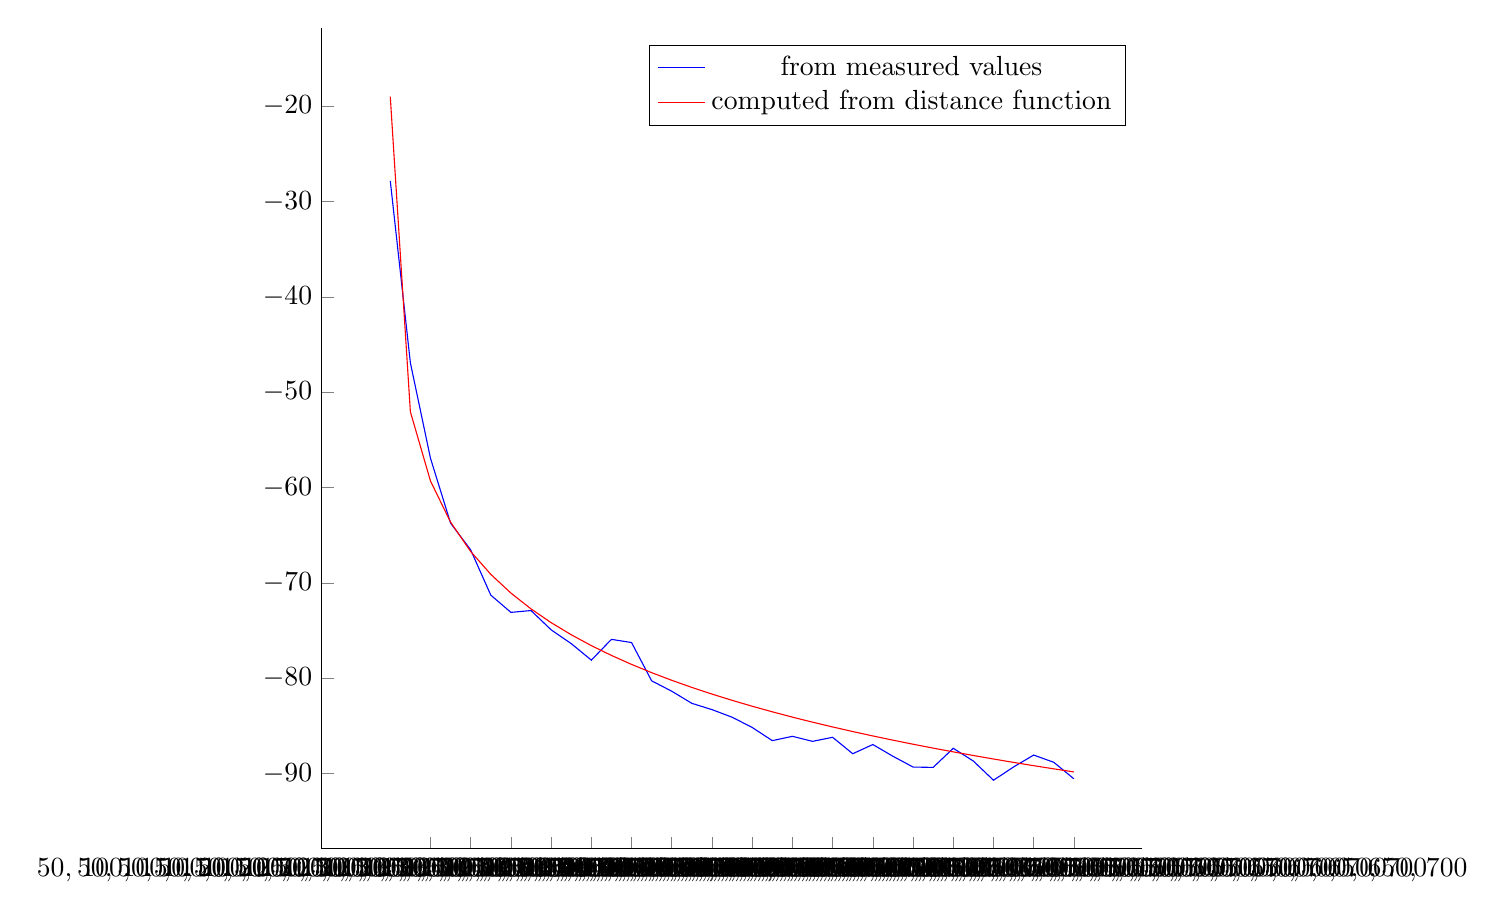
\begin{tikzpicture}
    \begin{axis}[
        no markers, axis lines*=left,
        %enlargelimits=false,
        %xlabel=Average RSSI, ylabel=Probability density,
        height=12cm, width=12cm,
        domain=0:700,
        xtick={2, 4, 6, 8, 10, 12, 14, 16, 18, 20, 22, 24, 26, 28, 30, 32, 34},
        xticklabel={50, 100, 150, 200, 250, 300, 350, 400, 450, 500, 550, 600, 650, 700}
        %stack plots=y
        %% xtick={4,6.5}, ytick=\empty,
        %grid=major
        ]
        \addplot coordinates {(0, -27.83419307295505) (1, -46.92156862745098) (2, -56.93304535637149) (3, -63.736301369863014) (4, -66.5452865064695) (5, -71.28635682158921) (6, -73.09453302961276) (7, -72.90234375) (8, -74.92373923739237) (9, -76.3717791411043) (10, -78.10295857988166) (11, -75.9241773962804) (12, -76.25923546418247) (13, -80.27360515021459) (14, -81.36496350364963) (15, -82.63513513513513) (16, -83.29462875197473) (17, -84.08870967741936) (18, -85.16179337231969) (19, -86.54743083003953) (20, -86.0923076923077) (21, -86.62264150943396) (22, -86.19658119658119) (23, -87.91878172588832) (24, -86.95373665480427) (25, -88.18548387096774) (26, -89.31612903225806) (27, -89.3529411764706) (28, -87.34693877551021) (29, -88.68888888888888) (30, -90.69767441860465) (31, -89.3076923076923) (32, -88.05882352941177) (33, -88.81818181818181) (34, -90.55)};
        \addlegendentry{from measured values};

        \addplot coordinates {(0, -19.0) (1, -52.05548236834798) (2, -59.31959641799338) (3, -63.63324587526918) (4, -66.71212547196625) (5, -69.10803434456606) (6, -71.06963425791125) (7, -72.7304778163845) (8, -74.17064690079624) (9, -75.44196437172961) (10, -76.57990143551223) (11, -77.60980684212777) (12, -78.5504260643717) (13, -79.41601268345701) (14, -80.21765799762699) (15, -80.96416238984608) (16, -81.6626258101218) (17, -82.31885947481244) (18, -82.93768004764144) (19, -83.52312439189049) (20, -84.07860931550455) (21, -84.60705239589171) (22, -85.11096473669596) (23, -85.5925231347412) (24, -86.0536269093458) (25, -86.49594314668114) (26, -86.92094308248812) (27, -87.32993162766424) (28, -87.72407153140404) (29, -88.10440330975827) (30, -88.4718618000685) (31, -88.8272900044145) (32, -89.17145073797043) (33, -89.505036487141) (34, -89.82867779781962)};
        \addlegendentry{computed from distance function};
    \end{axis}
\end{tikzpicture}


% measured
%[(0, -27.83419307295505), (1, -46.92156862745098), (2, -56.93304535637149), (3, -63.736301369863014), (4, -66.5452865064695), (5, -71.28635682158921), (6, -73.09453302961276), (7, -72.90234375), (8, -74.92373923739237), (9, -76.3717791411043), (10, -78.10295857988166), (11, -75.9241773962804), (12, -76.25923546418247), (13, -80.27360515021459), (14, -81.36496350364963), (15, -82.63513513513513), (16, -83.29462875197473), (17, -84.08870967741936), (18, -85.16179337231969), (19, -86.54743083003953), (20, -86.0923076923077), (21, -86.62264150943396), (22, -86.19658119658119), (23, -87.91878172588832), (24, -86.95373665480427), (25, -88.18548387096774), (26, -89.31612903225806), (27, -89.3529411764706), (28, -87.34693877551021), (29, -88.68888888888888), (30, -90.69767441860465), (31, -89.3076923076923), (32, -88.05882352941177), (33, -88.81818181818181), (34, -90.55)]


% function
%[(0, -19.0), (1, -52.05548236834798), (2, -59.31959641799338), (3, -63.63324587526918), (4, -66.71212547196625), (5, -69.10803434456606), (6, -71.06963425791125), (7, -72.7304778163845), (8, -74.17064690079624), (9, -75.44196437172961), (10, -76.57990143551223), (11, -77.60980684212777), (12, -78.5504260643717), (13, -79.41601268345701), (14, -80.21765799762699), (15, -80.96416238984608), (16, -81.6626258101218), (17, -82.31885947481244), (18, -82.93768004764144), (19, -83.52312439189049), (20, -84.07860931550455), (21, -84.60705239589171), (22, -85.11096473669596), (23, -85.5925231347412), (24, -86.0536269093458), (25, -86.49594314668114), (26, -86.92094308248812), (27, -87.32993162766424), (28, -87.72407153140404), (29, -88.10440330975827), (30, -88.4718618000685), (31, -88.8272900044145), (32, -89.17145073797043), (33, -89.505036487141), (34, -89.82867779781962)]


% \begin{algorithm}[H]
%     \DontPrintSemicolon
%     \SetKwFunction{FLinkmodel}{Linkmodel}
%     \SetKwProg{Fn}{Function}{}{}
% 
%     \Fn{\FLinkmodel{links}}{
%         model $\leftarrow$ An unordered map with id as key and RSSI as % value\;\;
% 
%         \ForEach{$l$ $\in$ links}{
%             fading $\leftarrow$ 0\;
% 
%             \ForEach{$k$ $\in$ links}{
%                 \If{$k$ $\neq$ $l$ \KwAnd nodes($k$) $\cap$ nodes($l$) = % $\emptyset$}{
%                     \KwContinue\;
%                 }
%                 \ElseIf{$l$ $=$ $k$}{
%                     corr $\leftarrow$ 1\;
%                 }
%                 \Else{
%                     angle $\leftarrow \theta$($l$, $k$)\;
%                     corr $\leftarrow$ $r$(angle)\;
%                 }
%                 
%                 
%                 ran $\leftarrow$ Pick a random value from a gaussian % distribution with mean $=$ 0, and standard deviation $=$ 1\;
%                 fading $\leftarrow$ fading + ran $\cdot$ corr\;
% 
%             }
%             %\tcp{distanceFading $\leftarrow l_d$($d$($l$))}
%             model[l.id] = $tx_{power}$ - (fading)\;
%         }
%     }
%     \caption{Pseoducode for the linkmodel}
%     \label{algo:linkmodel}
% \end{algorithm}
% \smallbreak
% 
% $d(link)$ computes the distance of a link.
% 
% $\theta(l, link2)$ computes the angle between two links.
% 
% $r(angle)$ is the autocorrelation function.

%$l_d(distance)$ computes the pathloss for the distance dependent part.

%\begin{algorithm}[H]
%    \DontPrintSemicolon
%    \SetKwFunction{FCorrelation}{Correlation}
%    \SetKwProg{Fn}{Function}{}{}
%
%    \Fn{\FCorrelation{angle}}{
%        \If{angle > 180}{
%            angle $\leftarrow$ 360 - angle\;
%        }
%
%        \Return angle / 180\;
%    }
%
%    \caption{Pseoducode for the Correlation}
%    \label{algo:correlation_func}
%\end{algorithm}